\noindent
\section{Diffusion model}
\label{diffusion_model}
% \begin{figure*}
%  \centering
%  \includegraphics*[scale=0.35]{figs1/diffusion.eps}
%  \caption{\label{diff_mod} Diffusion model: A is infected while B, C, D are susceptible ($k=2$). At t=1 A communicates with C. At t=2 A communicates 
%  with D. At t=3 A again communicates with C. At this point C has communicated with an infected individual (A) twice. So C becomes infected and would remain so 
%  for the whole duration of the diffusion process.}
% \end{figure*}


% Here we describe the overall framework and information diffusion technique
% that we assume for the rest of our study. 
%We assume a network network topology $G = <V,E>$ where $V$ represent the set of nodes and $E$ represent a set of edges between the nodes.
 
\if{0}
Our framework essentially resembles the Susceptible-Infected (SI) epidemic spreading model where we assume
a node can be in one of the two states - (i) susceptible or (ii)
infected. Susceptible nodes are the ones which do not have the
information or are not infected but can get infected if they come in contact
with an infected node. Similarly, an infected node is one which
already have the information and at each discrete time step randomly
selects one of its neighbors and tries to infect it. Note that we use the terms 
information and infection interchangeably as they essentially denote the
same thing in the context of the current study. 
%Since the model is motivated from the idea that an individual requires persuasion
%from the adopters before she adopts an idea, we quantify persuasion by the
%number of contacts she makes with the adopters in the network.
%Infected nodes are the oneswith the information and are trying to spread it while susceptibles are the ones without the information and can only receive it from an infected node.
\fi
 \begin{figure}[htpb]
 %\vspace{-0.8cm}
  \centering
  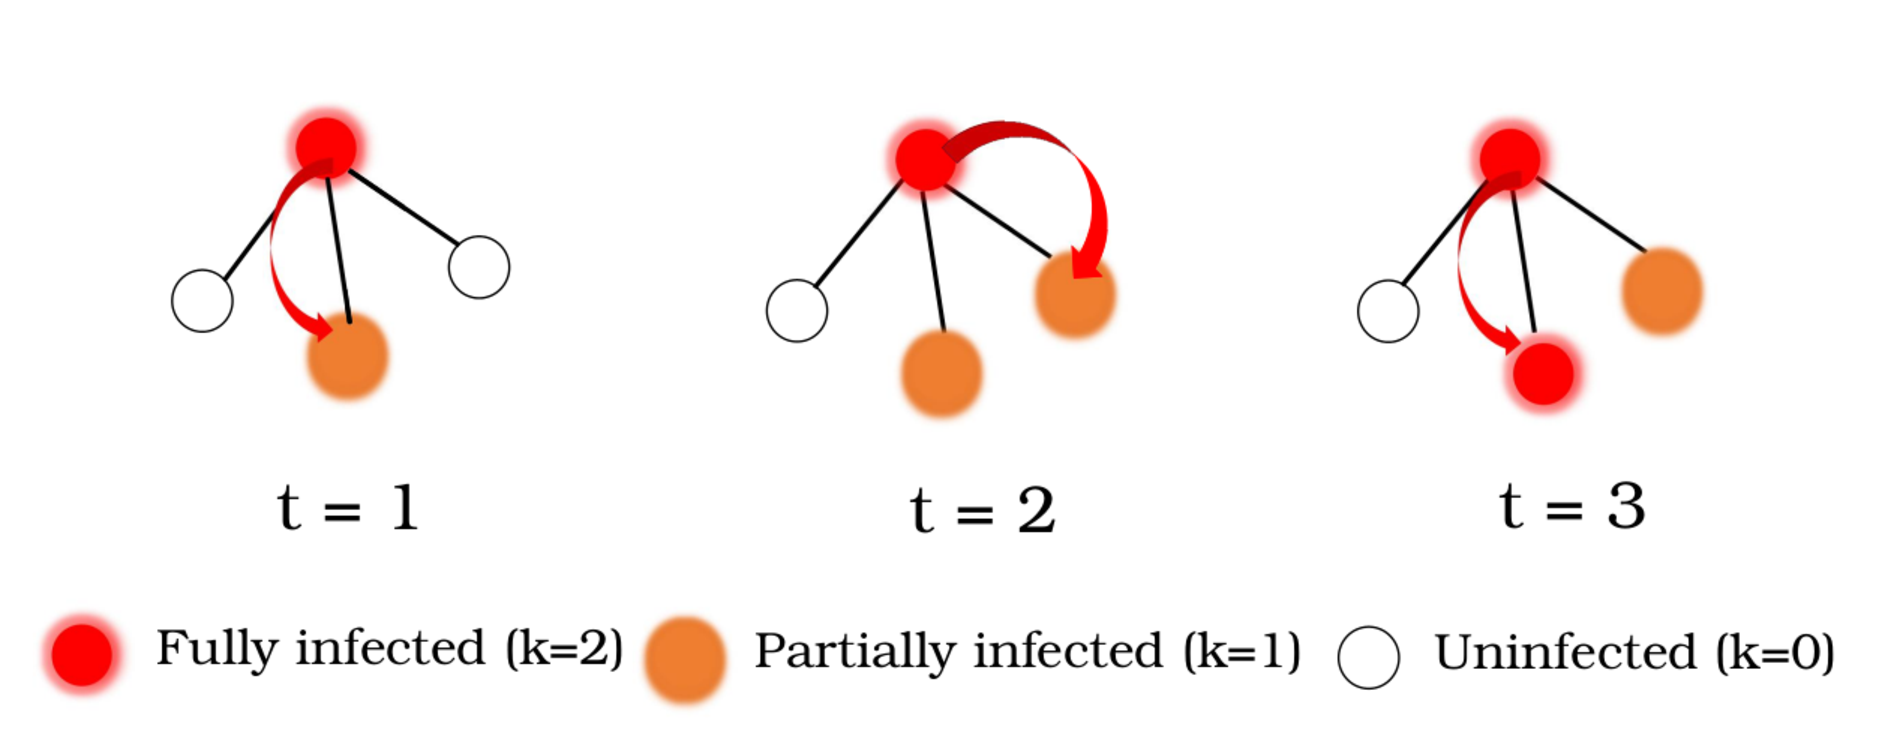
\includegraphics[scale=0.37]{./texfiles/Chapter_3/epl/figs1/dynamics.pdf}
  %\includegraphics*[scale=0.28]{figs1/plot_var_k.eps}
 %\includegraphics*[scale=0.15]{figs/T1_vs_exp_T1_d_reg.eps}
 
%\hspace{5mm}(a)\hspace{75mm}(b) 
%\vspace{-2mm}
 \caption{\label{fig_dynamics}Proposed diffusion model for $k=2$.}
 %\vspace{-.5cm}
\end{figure}
 
 
 \begin{figure}[htpb]
 %\vspace{-.5cm}
  \centering
  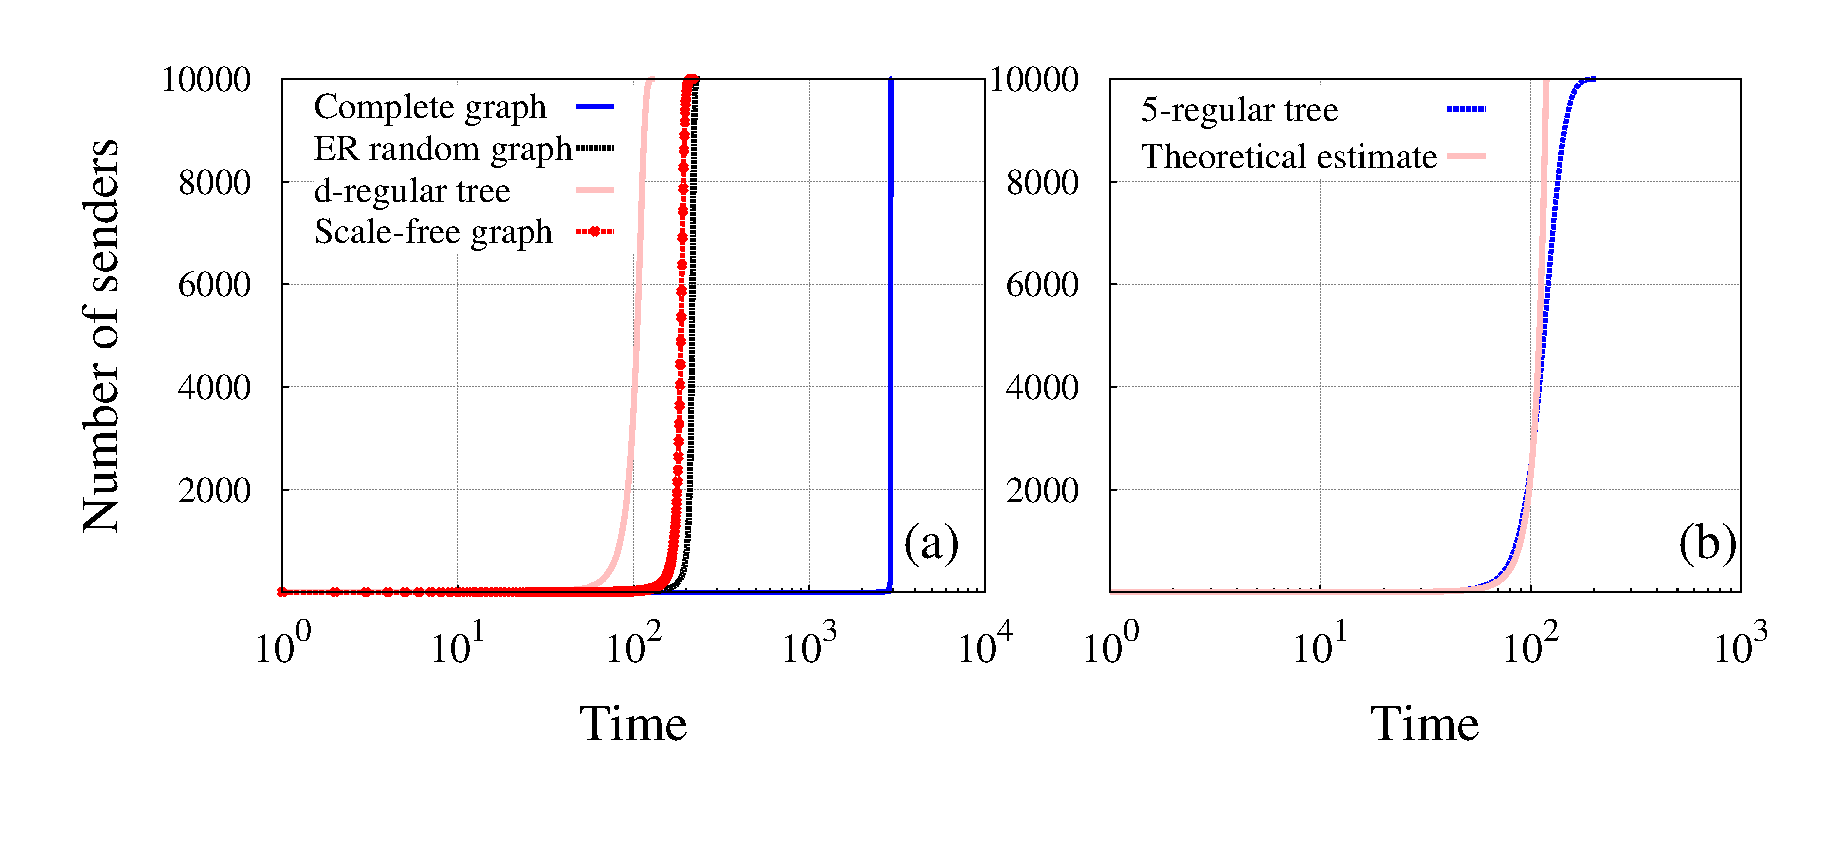
\includegraphics[scale=0.38]{./texfiles/Chapter_3/epl/figs1/plot_all.eps}
  %\includegraphics*[scale=0.28]{figs1/plot_var_k.eps}
 %\includegraphics*[scale=0.15]{figs/T1_vs_exp_T1_d_reg.eps}
 
%\hspace{5mm}(a)\hspace{75mm}(b) 
%\vspace{-4mm}
 \caption{\label{fig1} (a) The number of senders versus time steps for different network topologies (For ER random graph $p$ is $0.005$, for $d$-regular graph $d=5$ and for BA scale-free graph $m$ i.e., number of edges to attach from a new node to existing nodes is $5$) and 
 (b) The theoretical estimate and the simulated result for $d-$regular trees. The theoretical eastimate is obtained from equation 17.}
 \vspace{.5cm}
\end{figure}
 
% \todo{In figure~\ref{fig1} caption, add the vlaue of $p$ for ER graph and $\lambda$ for the scale-free graphs.}
 
Formally, we consider a network topology $G$ = $(V,E)$ where $V$ represents the set of
nodes in the network and $E$ denotes the set of edges between any pair of nodes in $%
V $. We initially start with a single infected node in the system. We
further assume that for a susceptible node to get infected,  $k$ encounters
with infected nodes are required. To put it in a simple way we consider that
a message $M$ needs to be spread over a network and message $M$ consists of $%
k$  identical tokens. At each communication instance one token gets transmitted from an
infected node to the susceptible node. Therefore, number of tokens ($k$) in a
message corresponds to the number of contacts required for a susceptible
node to get infected. Note that for the rest of this chapter we will present
our diffusion model in terms of messages and tokens. 
%Since the infected nodes essentially pass on the tokens we term them as senders while the susceptible ones are the non-senders.  

We assume that at time $0$, there is only one sender (infected) node present in the
system and it acts as the {\em initiator} of the diffusion process. At each
discrete time step a sender node randomly selects one of
its neighbors and  there is a transfer of a token from the sender to the non-sender. A non-sender node becomes a sender only after it receives exactly $k$
tokens (refer to figure \ref{fig_dynamics}). 
The analytical
estimation of the diffusion time based on the underlying topology requires a
case-by-case examination.
We formulate both analytical and empirical results for two extreme variants (in terms of edge density) of networks (a) complete graphs (dense) and (b) infinite regular trees (sparse)
while for others we provide empirical
results with intuitive justifications.
%\todo{Can we have a small picture demonstrating the dynamics since this is a very novel concept? We can take a small network, $k=3$ and illustrate the spread in three time points -- $t=0$ where only one node is black (the initiator), some intermediate $t=t^{'}$ where we show the $k$ values for different nodes (none of which is yet $=3$) and then $t=t^{''}$ where the first sender is formed (one node has $k=3$). We have enough white spaces between figures which can be reduced to fit in this picture.}
\if{0}
%Note that this results in creation of a subgraph at each time step roughly resembling a temporal network. 
% Assuming such a diffusion model we study in detail the diffusion time (i.e.,
% the time from the start till the time when all the nodes in the network
% receive the information and the algorithm terminates) given an underlying
% network topology.
\fi
% \begin{figure}[htpb]
%   \centering
%   \includegraphics[scale=0.28]{figs1/plot_var_k.eps}
%   %\includegraphics*[scale=0.28]{figs1/plot_var_k.eps}
%  %\includegraphics*[scale=0.15]{figs/T1_vs_exp_T1_d_reg.eps}
%  
% %\hspace{5mm}(a)\hspace{75mm}(b) 
%  \caption{\label{fig_k} Number of nodes at each stage of infection versus time for complete graph \todo{write more detailed description}}
% \end{figure}


\if{0} 
% \subsection{Agent configuration and network setup}
% 
% We consider a network topology $G = < V,E >$ where each node in $V$ represents an agent of the network and any link in $E$ represents a contact 
% opportunity between a pair of nodes (agents) in the whole time span through which the network is active. So for any node (agent) $n_{i}$ in this network, its one hop 
% neighbors are the nodes (agents) which are within the connection proximity of $n_{i}$ and at each time step $n_{i}$ at random can connect to any one of them. 
% 
% 
% \subsection{Information configuration}
% 
% As we stated earlier, we consider that the information diffusion occurs in parts. 
% We consider that thdie whole information $\mathcal{M}$ is divided into a set of $m$ tokens, i.e., $|\mathcal{M}| = m$ and in 
% a contact opportunity a single token gets transmitted.
%  We can also extend it to knowledge diffusion or special cases of disease spreading where a susceptible node gets infected 
%  only after it meets infected individuals for specified number of times. In these cases the total number of tokens 
%  would refer to the number of times ($m$) a susceptible (novice) individual communicates with an infected (knowledgeable) individual 
%  before it itself gets infected (knowledgeable). It can further be interpreted as the number of times a node should be reminded of an 
%  information before it remembers and participates in the diffusion process. Note that throughout our analysis we will stick to the 
%  notion of information and tokens for simplicity. 
% 
% 
% \subsection{Information diffusion technique}
% 
% In this framework, transfer of a message during a contact refers to the transfer of one single token of the information. 
% Transfer of a token from $u_i$ to $v_j$ during a contact can take place only 
% when $u_i$ qualifies as a {\em sender} by having all the tokens of the information.
% We mainly consider the $push$ technique of information diffusion which is described below. 
% 
% 
%  \noindent \emph{Push technique:} 
%   \begin{itemize}
%  % \vspace{-3mm}
%    \item \emph{Step 1:} At any time step, $u_i$ (already a sender) establishes a communication link with $v_j$, 
%    from its neighborhood and finds an exclusive set of tokens that $u_i$ has but $v_j$ does not have in its buffer. 
%    \item \emph{Step 2:} If $u_i$ can find such a (non-empty) set, then it transfers only one token from this set to $v_j$. 
%   \end{itemize}
% 
% Next we describe the information diffusion technique which we call $Blind Push$ (B-P) in detail.
% An initiator node is the one which has the full information in the beginning. At each time step all the nodes 
% in the system having the full information communicate with a node in their proximity and try to $push$. 
% %If it is successful then a unit bandwidth is consumed otherwise it is counted as wastage. 
% At the end of each time step all the nodes which have received all the tokens qualify as sender in the next time step. The algorithm terminates 
% when all the nodes in the system have the full information.
% We consider two types of epidemic processes - a) Susceptible-Infected (SI) and b) Susceptible-Infected-Recovered (SIR). 
% Susceptible nodes are the ones having a subset ($S$) of all the tokens ($0\leq |S| < m$, partial information) and the infected nodes are the one with 
% all the tokens (full information). The recovered nodes are the ones, which after having received the full information and spreading it for some time 
% have moved out of the system and is no longer part of the network.
% The information diffusion technique is similar for both the process. 

% \begin{algorithm}
% \caption{Blind Push (B-P)}\label{bp}
% \begin{algorithmic}[1]
% %\Procedure{MyProcedure}{}
% \STATE $select \, initiator$
% \STATE $make \, it \, sender$
% %\BState \emph{top}:
% %\If {$i > \textit{stringlen}$} \Return false
% %\EndIf
% %\State $j \gets \textit{patlen}$
%  \WHILE {$( not \, all \, nodes \, in \, the \, network \, have \, the \, message )$}
%  \FOR {$(each \, node \, which \, is \, already \, a \, sender)$}
% \STATE $select \, a \, node \, from \, its \, proximity;$
% \STATE $perform \, Push$;
% \IF {$(Push \, unsuccessful)$}
% \STATE $wastage;$
% \ELSE 
% \STATE $unit \, bandwidth \, consumed;$
% %\State $i \gets i-1$.
% %\State \textbf{goto} \emph{loop}.
% %\State \textbf{close};
% \ENDIF
% \ENDFOR
% \STATE $modify \, the \, list \, of \, senders;$
% \STATE $increment \, time;$
% \ENDWHILE
% %\EndProcedure
% \end{algorithmic}
% \end{algorithm}

% \subsection{Metrics of interest}
% %\vspace{-2mm}
% We are interested in evaluating the spreading model in terms of the following metrics-
% \begin{itemize}
% %\vspace{-4mm}
%  \item \textbf{Diffusion time $T^*$} - this is the time from the point when the message source starts the diffusion process to the point when all the agents in the network have received the the total information. 
%  $E(T^*)$ denotes the expected diffusion time. In addition, we are also interested in the time $T_i$ which is the minimum time at which there are $i$ senders (except the source) in the network, and especially in $T_1$ since, as we shall see, that this is the prime determinant of the entire broadcast time. 
% %\todo{why are these lines needed - Finally, note that $T^*$ may not correspond to $T_{n-1}$, i.e., the time when there are $n-1$ senders (except the source) in the network because all $n-1$ agents need not become senders to spread the message.}  
%  \item \textbf{Diffusion threshold} - 
% \end{itemize}
% \subsection{Dynamic topology}
% %\vspace{-2mm}
% We performed our experiments on synthetic topologies like complete graph, regular tree, regular graph and random graph. 
% A topology specifies the potential neighborhood of a node 
% - a node at each time step connects randomly to one of these nodes. A complete graph 
% topology would indicate that the 
% node can connect to any other node in the network while for other sparser topology it would 
% connect only to a subset of them.

\medskip
\fi
